%@author Brandon Roberts, Nate Olderman, Billy Rathje, DJ Maguddayao, Kyle Dybdal
%@date 9/23/13

\documentclass[12pt]{article}
\usepackage{graphicx}

\begin{document}

%-------------------------------------------------------------------------------------------------------------
% TITLE PAGE
%-------------------------------------------------------------------------------------------------------------

\begin{titlepage}
	\vspace*{\fill} %leave out given verticle space in a document
	\begin{center}
		{\Huge Story Creator Intermediate Report}\\ [0.5cm]	%make title huge and have .5cm space in between
		{\Large Brandon Roberts, Nate Olderman, Billy Rathje, DJ Maguddayao, Kyle Dybdal}\\[0.4cm]
		\today %put the date that the data is compiled
	\end{center}
	\vspace*{\fill}
\end{titlepage}

%------------------------------------------------------------------------------------------------------
%DESIGN SPECIFICATION
%----------------------------------------------------------------------------------------------------
\section{Design Specification}
	\subsection{Flow of Events}
	
The Story Creator module will be utilizing the Object Creator module, Visual Editor module, and the Animation modules work through the Sharing Framework.\\

The Sharing Framework will provide a database of the objects that were given to it by the Object Creators and a canvas to display the entire view.  These objects will be in the form of a .png and have a file that contains the methods and attributes that work for the particular object.  We will use the object .png itself to be placed on the story frame in order to display it to the storyteller.  To do this we will retrieve the information about the object from the Sharing Framework and then use the drawObject(...) method in order to display it on the frame.  Specifically we will be setting the original position where the object appears on the story panel.  \\

After the object is present on the story panel we will retrieve methods provided by the Visual Editor that were selected and edited by the storyteller.  We will then allow the storyteller to provide the parameters to these methods by the use of a drop down menu or by typing in the exact value (in the visual editor frame) they wish the method to use.  We will take the methods with parameters from the Visual Editor module and add the time that the user specified the action to occur.  The objects and their methods will be sent to the Animation module in a JSON format to interact with the objects at the specified time.  \\

\subsection{Interfaces and Code Flow}

\begin{verbatim}
Design Outline:

Sharing Framework interface
---Object and Methods 
------Provided interface for VE (objects and the methods they have)
---------Visual Editor interface for changing the methods 
-------------Create Specific Object with time and parameters 
----------Interface to take master object and make JSON object 
-------------Animation to move specified object 
\end{verbatim}


The Story Creator module will implement an interface made by the Sharing Framework in order to retrieve objects and their associated methods.  This will be a required interface because the sharing framework will need to provide methods for downloading images and JSON representations of methods developed in the visual editor. The Story Creation Framework will need to request data from the server - the server will not notify the Story Creation Framework when it receives new objects - which is why the interface is a required interface. The interface should include methods for downloading a .png by name, downloading methods for a .png by name, and getting the number of images and methods on the server. \\

The JSON methods and the png image downloaded from the server will need to be combined into an object. This will involve a 'master' object combining object data with new data developed in the process of making a story. The master object stores all information about objects on the canvas, including associated methods, animation timing, and the png file. As the storyteller works on the story, new information will be added to the fields about methods and animation timing. \\

The Story Creator module will utilize two interfaces for communicating with the Visual Editor. One is a provided interface that allows the visual editor to access which objects are on the canvas to attach methods to them. The other is a required interface that attaches methods developed in the Visual Editor to objects made in the canvas. This allows the objects downloaded from the server to be given new or updated methods. \\

We chose to use this architecture so that we would be able to easily retrieve the objects from the Sharing Framework as well as the methods that the objects can use.  It will then be very simple to combine the objects taken from the Sharing Framework interface and combine it with the storyteller modified methods that the Visual Editor interface will provide.  \\

We will then attach the specific time and parameters provided by the storyteller to the unique 'master' object that is created by the various components integrated in the story creator. \\ 

This 'master' object will be sent to the Animation Framework via a provided Animation Interface. The interface, provided by the Storyteller Framework, will allow the Animation Framework to access a JSON representation of the objects developed in the Story Creator. \\


%% Indents aren't working! I'll take a look later... -BR
\subsection{Detailed formal spec}
\begin{itemize}
	\item 'Master' Object Class (aka. 'StoryObject') \\
	The master object class includes all the data necessary for the Animation Framework to
	animate an object. It has fields for: \\

	\indent - Object's name ('name') \\
	\indent - Object's .png name ('pngName') \\
	\indent - Object's Methods (Array of string 'methods') \\
	\indent - Object's Timing Parameters (Dictionary of 'methods' at 'times') \\
	
	It should have the following methods: \\
	\indent - "String getJSONRepresentation(String name)" -- Makes JSON representation of object named 'name' \\
	\indent - Getters and setters for each field \\
	
	\item Required Sharing Framework Interface
	The Sharing Framework interface is a required interface that the Sharing Framework must make available to the Storyteller Framework for downloading objects and their associated methods, specified in JSON, from the server \\
	
	Methods: \\
	\indent - fileHandle getPngObject(String name) -- Returns a .png file with the name, "name," from the server. Throws an exception if the file does not exist. \\
	\indent - String getJSONMethodsForObject(String name) -- Returns a JSON file with the methods associated with the object named, 'name'. \\
	\indent - int getNumberOfImagesAndMethods() -- Returns the number of images and methods on the server. Useful for iterating through all images and/or methods. \\
	
	\item Required Visual Editor Interface \\
	The Visual Editor interface is an interface that the Visual Editor Framework must implement to communicate methods developed by the programmer to the Story Teller Framework. When the programmer develops new methods for an object or changes an object's methods, these methods must be attached to the object in the canvas. This interface allows the Story Teller Framework to access a JSON representation of the new methods. \\
	
	Methods: \\
	\indent - String getJSONRepresentationOfMethods(String storyObjectName) -- Returns a JSON representation of the new methods developed in the Visual Editor for the object named, 'storyObjectName'. \\
	
	\item Provided Visual Editor Interface \\
	The Storycreator Framework will provide the Visual Editor Framework with an interface for accessing objects currently on the canvas for which it can develop new methods. The Visual Editor framework will most likely first call getAllObjectsOnCanvas to see which objects are currently on the canvas, then it will call getJSONRepresentationOfMethods for one of the available objects to get a JSON representation of the methods already attached to the given object.  \\
	
	Methods: \\
	\indent String[] getAllObjectsOnCanvas() -- Returns an array of 'master' objects corresponding to all the objects on the canvas. \\
	
	\indent 	 String getJSONRepresentationOfMethods(String storyObjectName) -- Returns a JSON representation of the methods currently attached to an object named 'storyObjectName'. The reverse of the method in the required interface. \\
	
	\item Provided Animation Interface \\
	The Animation Framework will need to access JSON representations of the 'master' object, which contains all timing, method, and other information for each object in the canvas. The interface is fairly straightforward: \\
	
	Methods: \\
	\indent - String getJSONRepresentationOfStoryObject(String storyObjectName) -- Returns a JSON representation of the StoryObject named 'storyObjectName' with all the information necessary for the Animation Framework to animate the object. \\
	
\end{itemize}

\subsection{Design interface}
We have no interface.  We will be implementing the Visual Editor interface in order to retrieve the parameters for modified methods.

\subsection{Design details and restrictions}
We will begin every file name with "sc."  We will also need a folder for each component of the system (Visual Editor, Sharing Framework, Object Creator, and Animation Framework).  The Story Creator will also place the .png of the object in a folder labeled by name for that object.  This folder will contain another folder for all of the methods for the specific object(named by "objectNameMethods").  Where applicable we will also use camel casing instead of using underscore. 

\newpage
\subsection{UML}
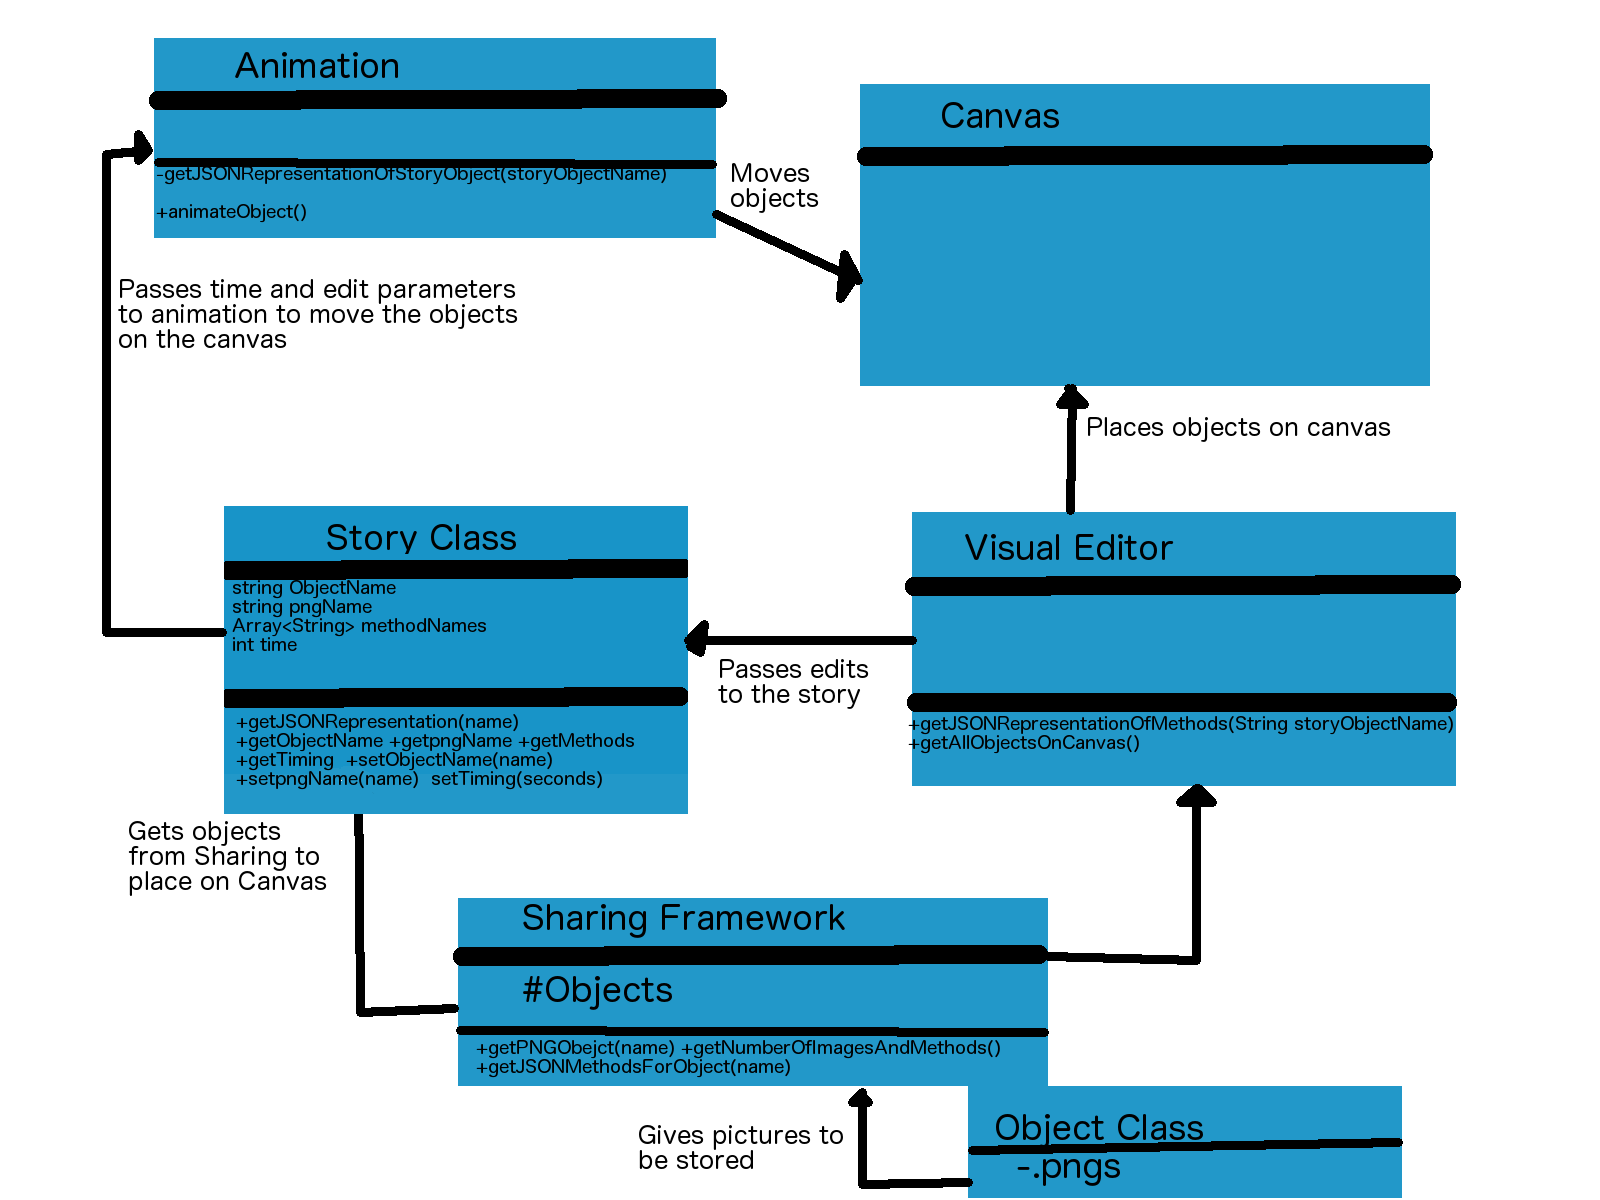
\includegraphics[scale=0.26]{Story_Creator_UML}
\\*
\\*

%------------------------------------------------------------------------------------------------------
%PROJECT STATUS
%----------------------------------------------------------------------------------------------------
\section{Project Status} 
\subsection{Current State of Project}
The state of the Story Creator segment of Edith is currently still in the planning stage. In favor of making clear the responsibilities of our team we have worked mainly on notes and documentation of what we plan to implement.

\subsection{Member Contribution}
So far all team members have provided a contribution on all notes and documentation done, whether it be through the actual action of taking notes, creating detailed charts and graphs, and/or providing ideas and information that help clarify the process. For further implementation of the project the team members have agreed to discuss what components need to be done when, and distrubute the work according to availabilities and specialties.

\subsection{Previous Development Process}
As previously mentioned, the development process to date has been mostly collaborative on all work. For this work we mostly would take advantage of LaTeX for pdf generation and github in conjunction with e-mailing for collaboration. This procedure has proven to be very effective, especially in contrast to our initial idea of just working when in class, which was dismissed very early on. \\
If given the chance to redo the project from the beginning, we feel that we would change how early we start the work and the attention we paid to the small details. \\
The only challege we have met so far has been a struggle to understand and clarify the overall concept of our module. Through hard work and communication with Joel Ross we have gained clarity that should help us carry on further. \\

\subsection{Timeline for Implementation}
\begin{figure}
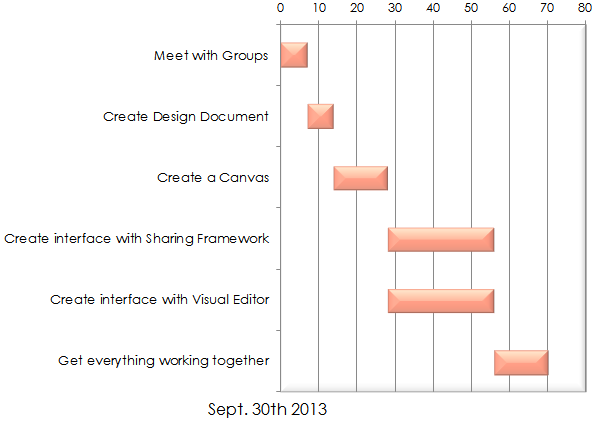
\includegraphics{GanttChart.png}
\caption{Gantt Chart}
\end{figure}



%------------------------------------------------------------------------------------------------------
%
%----------------------------------------------------------------------------------------------------
\end{document}